\chapter{Contesto aziendale}

\section{Dominio applicativo}
% Breve introduzione al settore del \textit{Enterprise Application Integration}, al tipo di clientela (ovvero pubblica e privata di grandi dimensioni, big data), alla tipologia di \textit{software} prodotti dall’azienda per la clientela (\textit{Middleware}), e alla propensione all’innovazione (richieste da parte della clientela
In conclusione al percorso di studi del corso di laurea in Informatica ho effettuato lo \textit{stage} presso \textit{Sync Lab}.
Sync Lab è un'azienda di produzione \textit{software} e integrazione di sistemi che fornisce principalmente prodotti a clienti di grande dimensione, sia pubblici che privati.

L'azienda è suddivisa in molteplici settori con diverse sedi; l'esperienza personale mi ha portato a conoscere il settore dell'\textit{Enterprise Architecture Integration} e del \textit{Tecnical Professional Services Padova}.
Il percorso di \textit{stage} intrapreso è associato al primo di questi, che si occupa principalmente dell'EAI (\textit{Enterprise Application Integration}) ovvero dell'integrazione funzionale di applicazioni aziendali per una clientela di grandi dimensioni (come un'azienda di telecomunicazioni), tramite sistemi di integrazione \textit{Middleware}.
I \textit{Middleware} prodotti comprendono l'utilizzo di molteplici linguaggi e tecnologie in continua evoluzione.
% Il caso d'uso realizzato nel mio percorso ha simulato un grande cliente gestore di telecomunicazioni, secondo una visione coerente con il tipo di clientela reale dell'azienda.

Questo contesto dell'integrazione aziendale presenta un'importante propensione all'innovazione, talvolta esplicitamente richiesta dai clienti.
Una direzione dell'evoluzione attuale nel settore EAI riguarda la migrazione verso sistemi sempre più distribuiti, in grado di gestire efficacemente ed in tempo reale flussi di dati in continua crescita.
L'avanguardia tecnologica è pertanto uno dei principali temi dell'azienda, che garantisce che essa rimanga sempre competitiva sul mercato dei sistemi di integrazione.

% \bigskip\noindent
% Esposizioni delle ragioni personali che hanno portato alla scelta di tale percorso.


\section{Processi interni e strumenti organizzativi}

% Esposizione delle norme organizzative (\textit{online meeting}, \textit{smart working}, presenze in sede), degli strumenti utilizzati nel rapporto con l’azienda (chat, email e \textit{Project Board}), e delle norme di progetto.
%
% \bigskip\noindent
% Processi interni in cui sono stato coinvolto: Sviluppo, Collaudo, Verifica, Formazione, Manutenzione/Evoluzione.

% \bigskip\noindent
% Breve presentazione dei ruoli delle persone coinvolte nel percorso di \textit{stage}.

L'azienda adotta dei processi interni per delineare l'avanzamento di un progetto.
Durante il percorso di \textit{stage} sono stato coinvolto nei processi di Formazione, Sviluppo, Verifica e Collaudo; i processi di Manutenzione ed Evoluzione sono stati solamente accennati in quanto al di fuori dello scopo del percorso.
Questi processi, nella mia esperienza personale, non sono stati delineati rigorosamente, al fine di garantire una certa rapidità e adattabilità al progetto di sperimentazione.
Ogni processo è suddiviso in attività modulari, per rendere l'avanzamento efficace e quantificabile.

L'organizzazione efficiente di un progetto è garantita dall'utilizzo dei vari strumenti a supporto, quali \textit{Kanban Board} (come \textit{Click Up} per la gestione di progetto e \textit{Notion} per le prenotazioni della postazione di lavoro in sede), \textit{chat} (come \textit{Google Chat}) per i confronti rapidi con gli altri membri interni al progetto ed e-mail per le comunicazioni con componenti esterni al progetto.

Lo strumento più utilizzato in ambito organizzativo durante il percorso è la \textit{Kanban Board} di \textit{Click Up}, che ha permesso la gestione, il confronto, la quantificazione e la verifica del progresso.
Le figure seguenti illustrano alcuni \textit{screenshot} che raffigurano lo stato dell'avanzamento.

\bigskip
\begin{figure}[h]
  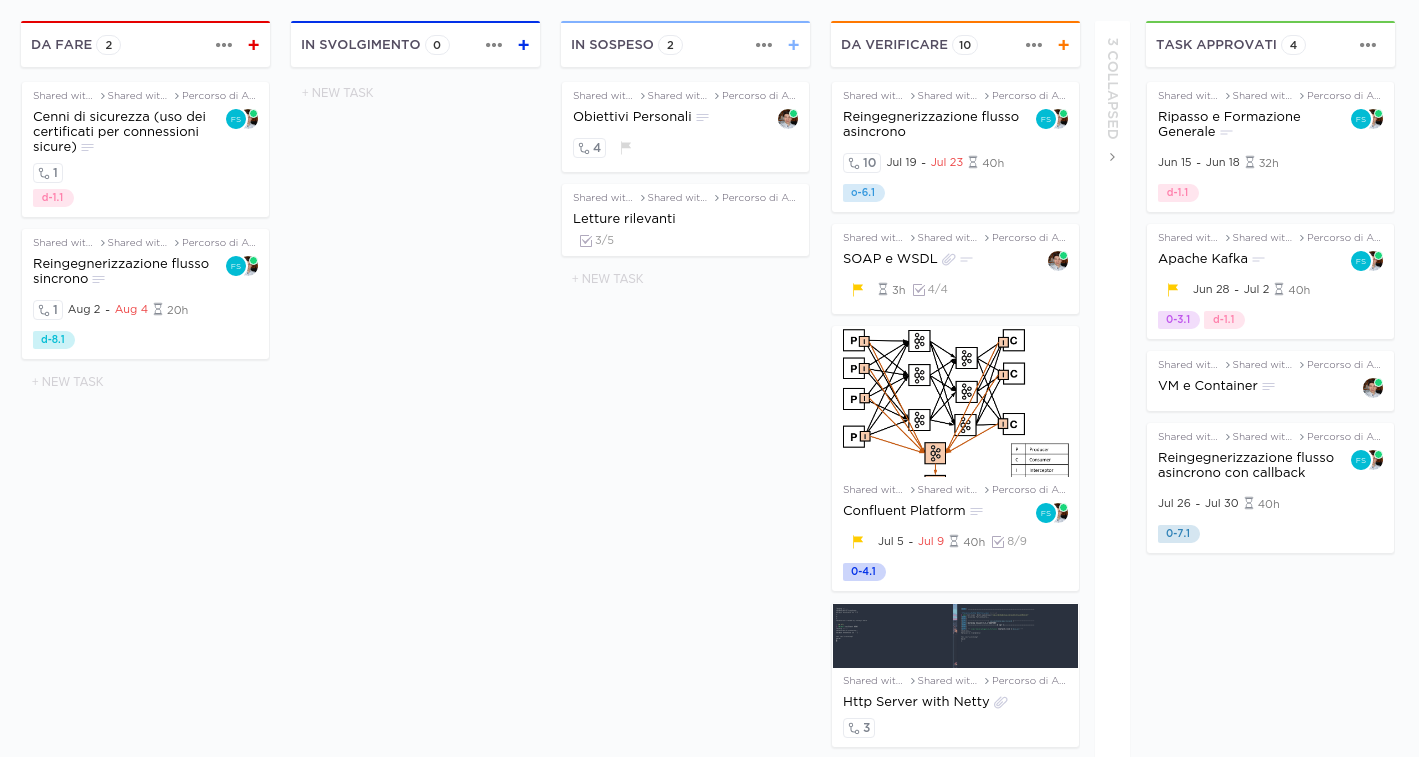
\includegraphics[width=\textwidth]{images/clickup_board_v2.png}\\
  \caption{\textit{Kanban Board} del progetto di \textit{stage}}
\end{figure}

Le attività (\textit{task}) vengono inizialmente create nella colonna "DA FARE" dal tutor aziendale o da me, ove ritenuto opportuno.
Per dimostrare l'avanzamento il \textit{task} si sposta verso destra a seconda dello stato raggiunto; lo stagista ha la responsabilità del cambiamento di stato fino alla colonna "DA VERIFICARE", dopodichè è compito del tutor aziendale la verifica e lo spostamento del \textit{task} in "TASK APPROVATI", che comporta l'approvazione finale e conclusione dell'attività.

Per tenere traccia del lavoro svolto riguardante una specifica attività ho utilizzato le \textit{card} messe a disposizione dalla piattaforma, che mi hanno consentito di delineare precisamente la pianificazione e descrizione dell'avanzamento in dettaglio del singolo \textit{task}.
Questa \textit{card} contiene una casella di testo per inserire una descrizione e appunti utili ove sia richiesto, una \textit{checklist} approfondita, e una colonna che mantiene uno storico dei commenti; quest'ultima colonna non solo permette a me di mantenere un'importante resoconto sul lavoro svolto, ma consente anche al tutor aziendale e esperti del settore di quantificare il progresso e di fornire un aiuto rapido e contestuale.

\begin{figure}[H]
  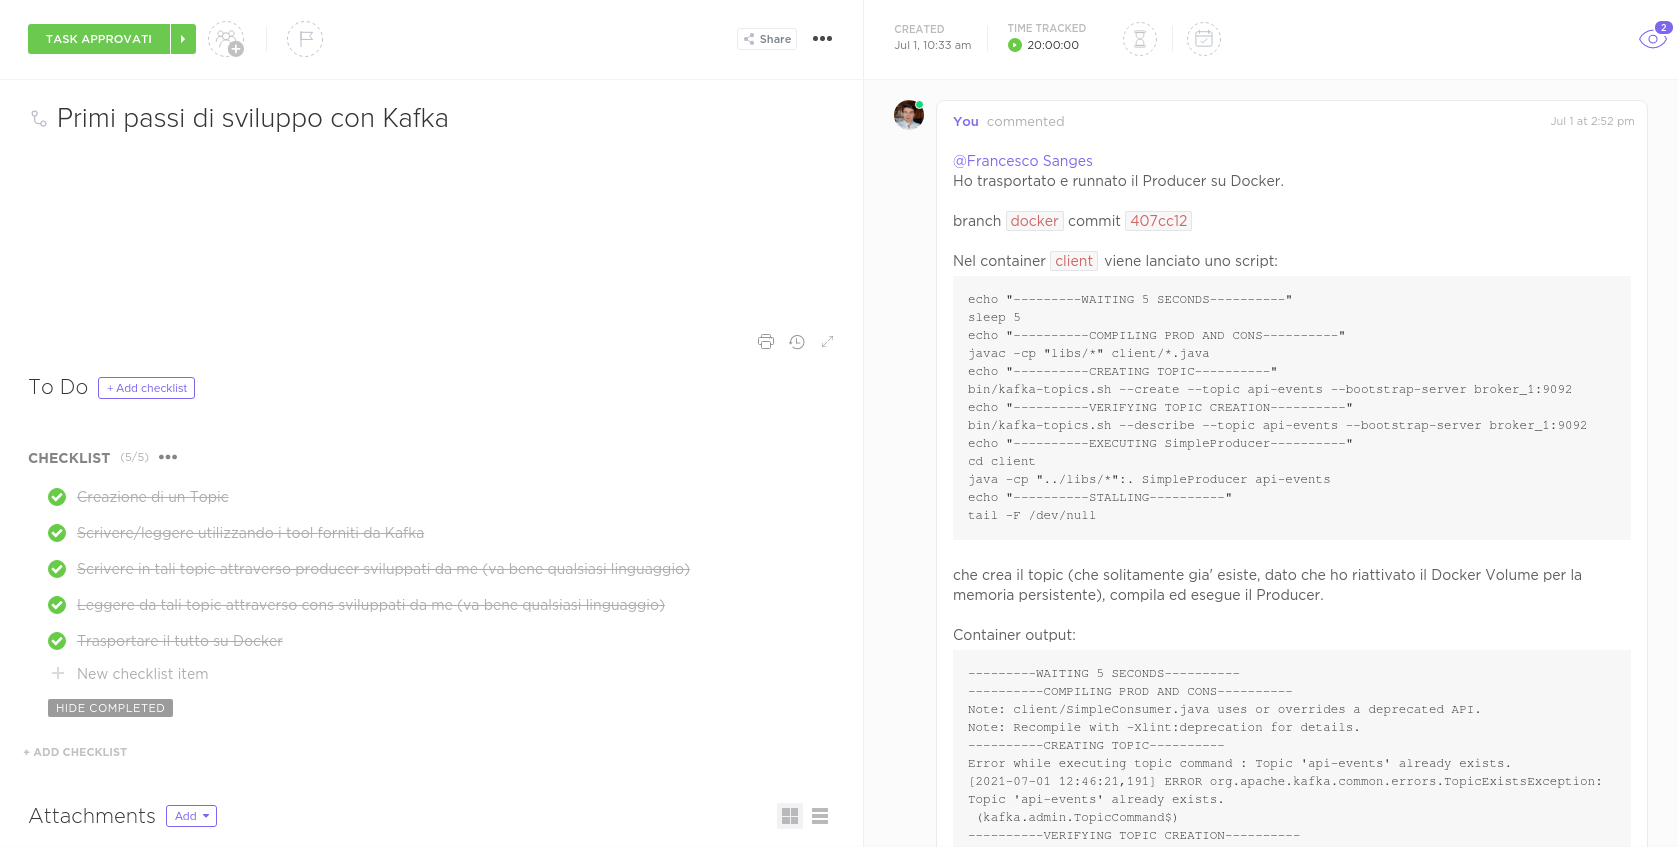
\includegraphics[width=\textwidth]{images/clickup_task_v2.png}\\
  \caption{Esempio di un'attività del processo di Formazione}
\end{figure}


\section{Ambiente di lavoro}

% Sviluppo indipendente dal sistema operativo, produzione di \textit{software} non strettamente legati ad uno specifico linguaggio, utilizzo di ambienti virtuali quali \textit{Virtual Machine} e \textit{container} per simulare sistemi indipendenti.
L'ambiente di lavoro di cui ho avuto esperienza risulta libero e flessibile.
Lo sviluppo del prodotto nell'ambito del EAI dev'essere indipendente dal linguaggio di programmazione, dagli strumenti utilizzati per l'esecuzione e sviluppo, e possibilmente anche dal Sistema Operativo su cui eseguire il \textit{software}.
A tal scopo si utilizzano strumenti quali \textit{Virtual Machine} e \textit{Container}: essi non solo garantiscono l'indipendenza dal Sistema Operativo in uso, ma simulano efficacemente il caso d'uso reale in cui i vari eseguibili sono dislocati in più computer o server come spesso accade per il cliente.

Nonostante il percorso formativo abbia visto l'apprendimento di entrambe le tecnologie tramite l'utilizzo dei \textit{software} \textit{Virtual Box} e \textit{Docker}, solo quest'ultima è stata utilizzata durante il progetto poiché più efficente e minimale.
Più precisamente, ho utilizzato l'estensione \textit{Docker-compose} per gestire in modo elegante la generazione e collaudo di più servizi indipententi: non solo questo \textit{software} consente di creare una rete di \textit{container} comunicanti, ma rende anche rapido ed efficaciente lo sviluppo grazie alla possibilità di modificare e riavviare un singolo servizio all'interno del sistema.
